% !TeX TXS-program:bibliography = txs:///biber
\documentclass[unknownkeysallowed]{beamer}
\usetheme{UniKlu}
\usepackage[backend=biber,style=apa,sorting=nty, bibencoding=utf8]{biblatex}
\addbibresource{/home/donkarlo/Dropbox/projs/research/refs.bib}


\usepackage{xcolor}

\title{Collective Self-awareness in Multi-Robot Systems}
\author{Mohammad Rahmani}
\institute{DECIDE Doctoral School}

\begin{document}
\begin{frame}
	\maketitle
\end{frame}

\begin{frame}{Self-awareness(SA) in Biological Intelligent Agents (IA)}
	A Biological IA is conscious/SA if
	\begin{itemize}
		\item It is born with an initial knowledge in the form of temporal cause-effect (Called experience from here)
		\item It has the ability to make a distinction between new experiences and old experiences. 
			\begin{itemize}
				\item The ability to make a distinction between known and unknown, if known can be built of different pieces of previous experiences (alphabet) otherwise it is unknown.
			\end{itemize}
		\item Memorize new experiences.
		\item Invoke the right experience whenever it witnesses the evidence. 
		\item This presentation only discusses detecting new experiences.
	\end{itemize}
\end{frame}


\begin{frame}{SA for single Artificial IAs}
	\begin{itemize}
		\item Should implement the aforementioned characteristics in a SA.
		\item The very first step is to introduce a model to encode the experiences including the initial experience.
	\end{itemize}
\end{frame}

\begin{frame}{An active-self IA}
	\begin{itemize}
		\item An approach in relating excteroceptive and proprioceptive data: 
		\item I cause something to happen in myself to see the effect over the course of time in the world outside
		\item Taking control data as proprioceptive sensory/cause/control/evidence data and position as exteroceptive sensory/effect/state data
	\end{itemize}
\end{frame}

\begin{frame}{An active-self IA}
	\begin{itemize}		
		\item A drone that knows how much it's position changes in space if it increases 10\% of it's front rotors
	\end{itemize}
\end{frame}

\begin{frame}{How to mathematically model - Bayesian Networks (BNs)}
	\begin{itemize}
		\item BNs are probabilistic models which model the probability of occurrence of an event conditioned on occurrence of some evidence. \item This builds the cause-effect section of a temporal, cause-effect model
			\begin{itemize}
				\item In the example in previous slide, this can be interpreted by the a drone as "How much change in position may I experience if I increase my front rotors' power by 10\%"
			\end{itemize} 
		\item DBNs take time into consideration by predicting an event not only based on the evidence but also based on the previous state of the IA 
			\begin{itemize}
				\item If the previous drone not only knows how much power it has added to its rotors but also what its current position is, then it can estimate its next position
			\end{itemize}
	\end{itemize}
\end{frame}


\begin{frame}{How to mathematically model - Bayesian Networks (BNs)}
	\begin{itemize}
		\item DBNs take time into consideration by predicting an event not only based on the evidence but also based on the previous state of the IA 
		\begin{itemize}
			\item If the previous drone not only knows how much power it has added to its rotors but also what its current position is, then it can estimate its next position
		\end{itemize}
	\end{itemize}
\end{frame}



\begin{frame}{How to mathematically model - Filtering}
	\begin{itemize}
		\item No (mobile) intelligent agent can never know what its true state is in continuous state space it can only estimate its state.  A bank of Kalman filters can map the observation to continuous state space.
		\item Known experiences of words of a dictionary can be composed of known alphabets. These alphabets can be built based on different strategies, but all should start by discretizing the (generalized) state space.
		\item Now we need another filter to map continuous estimated (generalized) state to meaningful(known, already seen) regions. To do this a bank of Particle filter can be used.   
	\end{itemize}
\end{frame}

\begin{frame}{How each DBN look like - Markov Jump Filter Model}
	\begin{figure}
		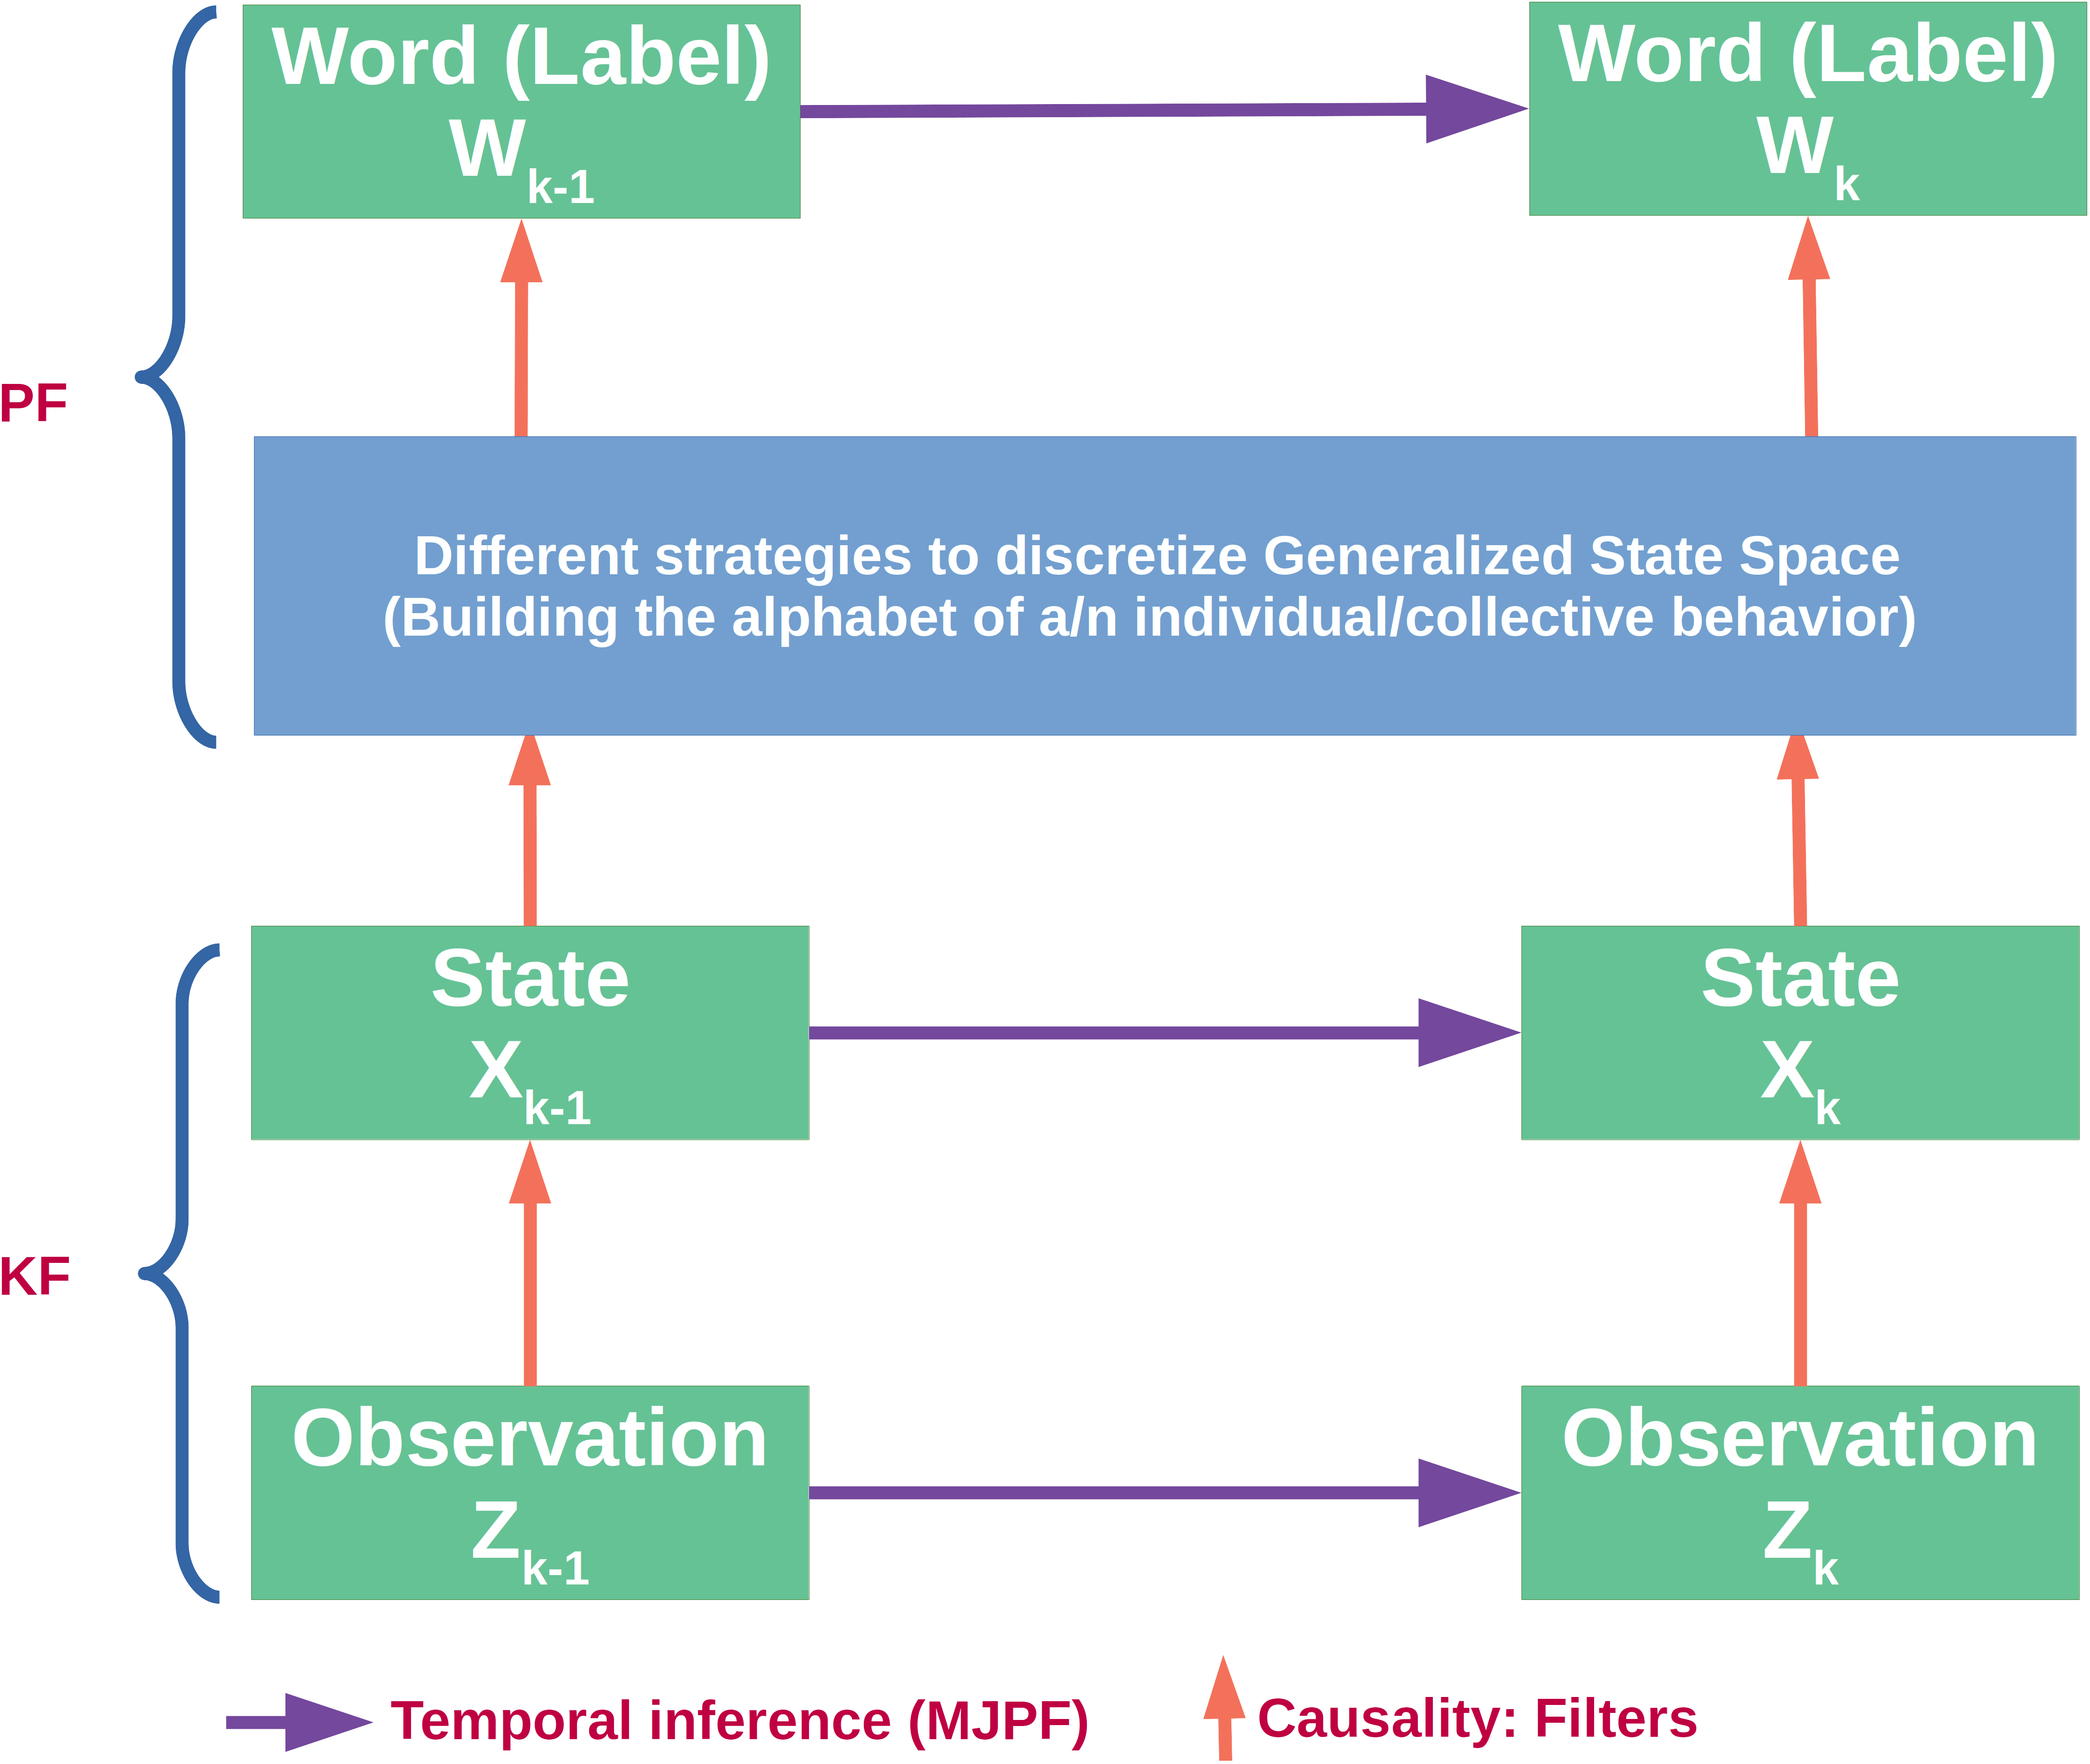
\includegraphics[scale=0.05]{/home/donkarlo/Dropbox/projs/research/artificial-intelligence/self-awareness/docs/assets/mjpf.png}
		\caption{}
	\end{figure}
\end{frame}

\begin{frame}{Example}
	\begin{figure}
		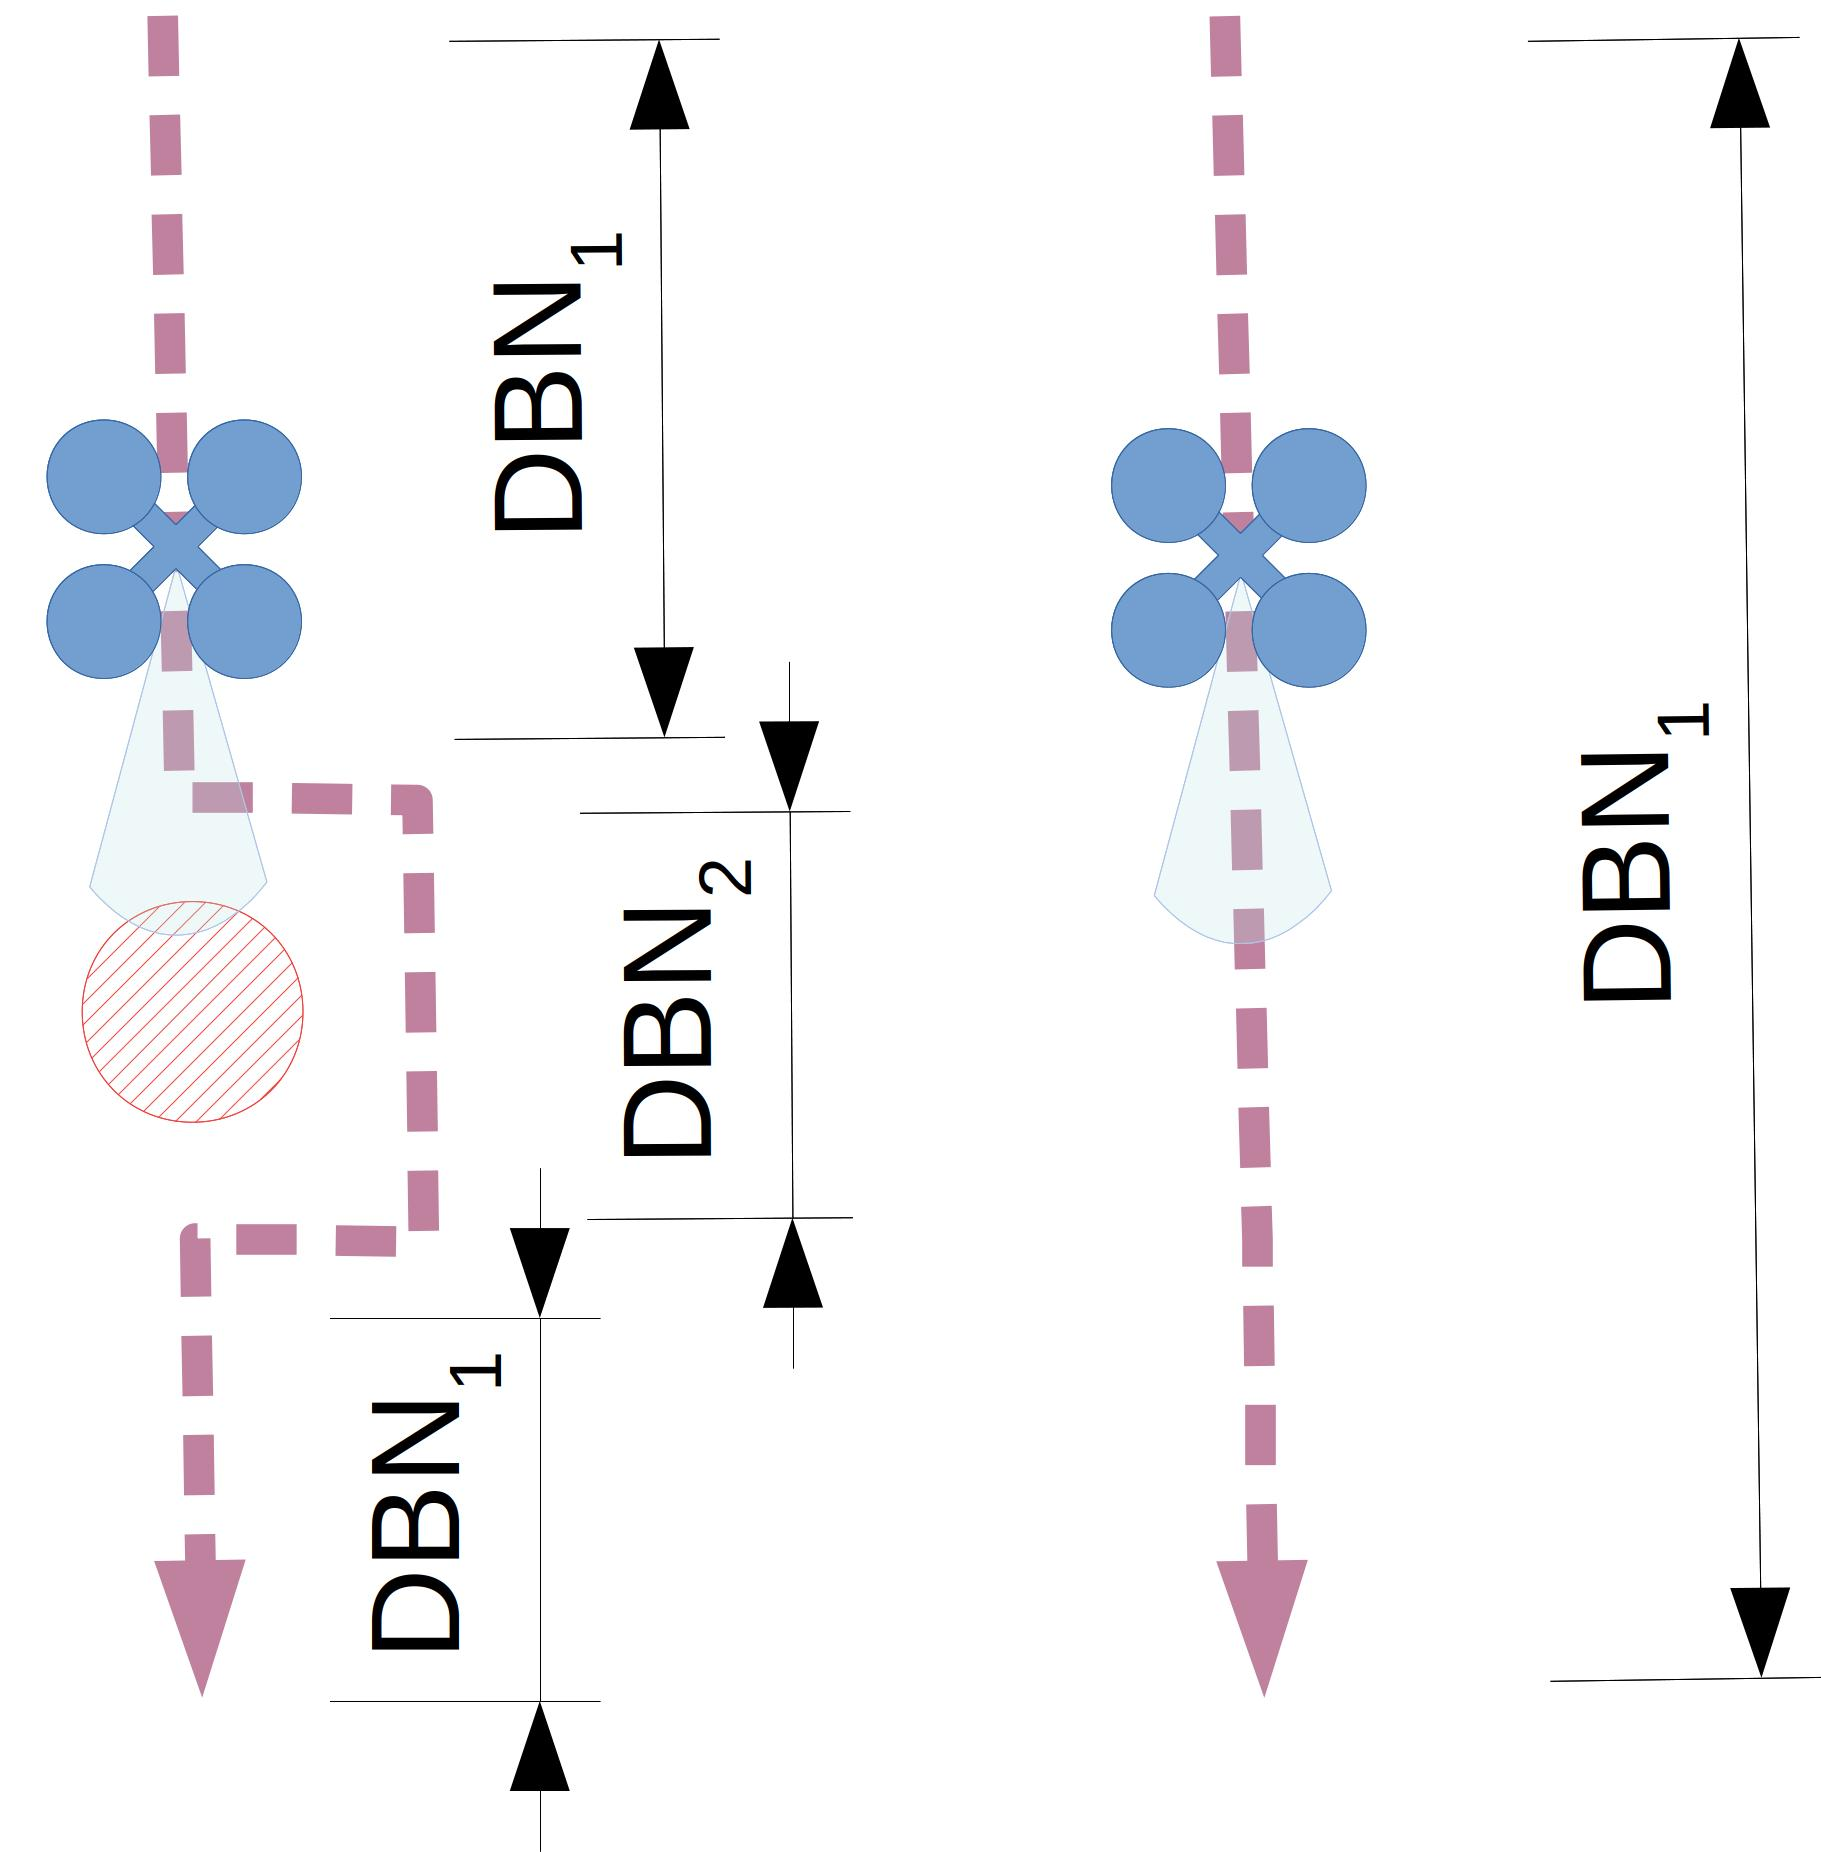
\includegraphics[scale=0.7]{/home/donkarlo/Dropbox/projs/research/artificial-intelligence/self-awareness/docs/assets/different-dbns.jpg}
		\caption{}
	\end{figure}
\end{frame}


\begin{frame}{The models choice}
	\begin{itemize}
		\item The choice of other the right DBN to practice is teh subject of another study but some research group are working on ideas from scientists such as Karl Friston\footfullcite{friston-2010-the-free-energy-principle-a-unified-brain-theory}
	\end{itemize}
\end{frame}

\begin{frame}{An example of previous works}
	\begin{figure}
		\includegraphics[scale=0.4]{/home/donkarlo/Dropbox/projs/research/assets/reg-car-pm.jpg}
		\caption{}
	\end{figure}
	\fullcite{kanapram-2019-dynamic-bayesian-approach-for-decision-making-in-ego-things}
\end{frame}

\begin{frame}{An exemplary previous work}
	\begin{figure}
		\includegraphics[scale=0.4]{/home/donkarlo/Dropbox/projs/research/assets/two-tasks.jpg}
		\caption{}
	\end{figure}
\end{frame}

\begin{frame}{An exemplary previous work}
	\begin{figure}
		\includegraphics[scale=0.4]{/home/donkarlo/Dropbox/projs/research/assets/three-d.jpg}
		\caption{}
	\end{figure}
\end{frame}

\begin{frame}{An exemplary previous work}
	\begin{figure}
		\includegraphics[scale=0.23]{/home/donkarlo/Dropbox/projs/research/assets/abnormality.jpg}
		\caption{}
	\end{figure}
\end{frame}

\begin{frame}{Collective SA}
	Can the same studies happen for the course of relationship between IAs?
	In \fullcite{baydoun-2019-prediction-of-multi-target-dynamics-using-discrete-descriptors-an-interactive-approach} a solution is proposed. 
	Force fields represent the normal course of relationship which should be maintained between two agents
	\begin{figure}
		\includegraphics[scale=0.3]{/home/donkarlo/Dropbox/projs/research/assets/two-relation-force-field.jpg}
		\caption{}
	\end{figure}
\end{frame}

\begin{frame}{Collective SA}
	A coupled, multilevel, switching DBN to describe the relationship 
	\begin{figure}
		\includegraphics[scale=0.3]{/home/donkarlo/Dropbox/projs/research/assets/mjpf-two.jpg}
		\caption{}
	\end{figure}
\end{frame}

\begin{frame}{Collective SA}
	Abnormality signals
	\begin{figure}
		\includegraphics[scale=0.25]{/home/donkarlo/Dropbox/projs/research/assets/two-abnormal.jpg}
		\caption{}
	\end{figure}
\end{frame}

\begin{frame}{Collective SA}
	Abnormality signals
	\begin{figure}
		\includegraphics[scale=0.25]{/home/donkarlo/Dropbox/projs/research/assets/two-abnormal-abnormal.jpg}
		\caption{}
	\end{figure}
\end{frame}

\begin{frame}{Collective SA - Future plan}
	As a future effort we seeks to apply the same idea for formation control of multiple drones
	\begin{figure}
		\includegraphics[scale=0.8]{/home/donkarlo/Dropbox/projs/research/assets/two-drones-relation-ship.jpg}
		\caption{}
	\end{figure}
\end{frame}

\begin{frame}[allowframebreaks]{References}
	\printbibliography
\end{frame}
\end{document}
